\section{Đề ôn thi giữa kỳ 2 toán 10}
\subsection{Phần trắc nghiệm}
Câu trắc nghiệm nhiều phương án lựa chọn. Học sinh trả lời từ
câu 1 đến câu 12. Mỗi câu hỏi học sinh \textit{chỉ chọn một} phương án.
\Opensolutionfile{ans}[Ans/Dapan]
\hienthiloigiaiex
%%%=============EX_1=============%%%
\begin{ex}%[0D3N1-3]%[Dự án đề kiểm tra Toán khối 10 GHKII NH23-24-Dot 2- Thái Bảo]%[Đề số 7 - KNTT]
	Cho hàm số $y=f(x)$ có đồ thị trên đoan $[-5; 5]$ như hình bên\\
	\begin{center}
		\begin{tikzpicture}[line join=round, line cap=round,>=stealth,thick]
			\tikzset{every node/.style={scale=0.9}}
			\draw[->] (-6.1,0)--(6.1,0) node[below left] {$x$};
			\draw[->] (0,-3.1)--(0,3.1) node[below left] {$y$};
			\draw (0,0) node [below left] {$O$};
			\foreach \x/\nx in {-5/-5,-4/-4,-3/-3,-2/-2,-1/-1,1/1,2/2,3/3,4/4,5/5}
			\draw[thin] (\x,1pt)--(\x,-1pt) node [below] {$\nx$};
			\foreach \y/\ny in {-2/-2,-1/-1,1/1,2/2}
			\draw[thin] (1pt,\y)--(-1pt,\y) node [below] {$\ny$};
			\draw[dashed,thin](-5,0)--(-5,-1)--(0,-1);
			\draw[dashed,thin](-2,0)--(-2,2)--(0,2);
			\draw[dashed,thin](2,0)--(2,-2)--(0,-2);
			\draw[dashed,thin](5,0)--(5,1)--(0,1);
			\begin{scope}
				\clip (-5,-3) rectangle (5,3);
				\draw[samples=200,domain=-5:-2,smooth,variable=\x] plot (\x,{1*(\x)+4});
				\draw[samples=200,domain=-2:2,smooth,variable=\x] plot (\x,{-1*(\x)});
				\draw[samples=200,domain=2:5,smooth,variable=\x] plot (\x,{1*(\x)-4});
			\end{scope}
		\end{tikzpicture}
	\end{center}
	Tập giá trị của hàm số $y=f(x)$ trên đoạn $[-5; 5]$ là
	\choice
	{$[-5; 5]$}
	{$[-1;1]$}
	{$[1;2]$}
	{\True $[-2; 2]$}
	\loigiai{}
\end{ex}
%%%=============EX_2=============%%%
\begin{ex}%[0D3N1-5]%[Dự án đề kiểm tra Toán khối 10 GHKII NH23-24-Dot 2- Thái Bảo]%[Đề số 7 - KNTT]
	\immini{Cho hàm số có đồ thị như hình bên. Khẳng định nào sau đây là \textbf{sai}?
		\choice
		{Hàm số nghịch biến trên khoảng $(-\infty;-1)$}
		{Hàm số đồng biến trên khoảng $(1;+\infty)$}
		{\True Hàm số nghịch biến trên khoảng $(-1; 1)$}
		{Hàm số đồng biến trên khoảng $(-1; 0)$}}
	{
		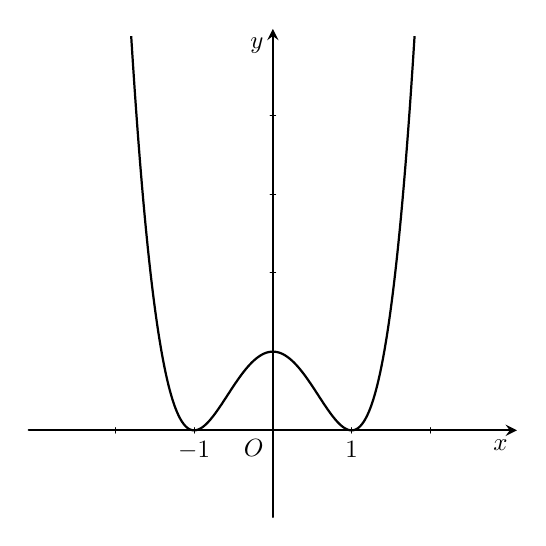
\begin{tikzpicture}[line join=round, line cap=round,>=stealth,thick]
			\tikzset{every node/.style={scale=0.9}}
			\draw[->] (-3.1,0)--(3.1,0) node[below left] {$x$};
			\draw[->] (0,-1.1)--(0,5.1) node[below left] {$y$};
			\draw (0,0) node [below left] {$O$};
			\foreach \y/\ny in {1/1,2/2,3/3,4/4}
			\draw[thin] (1pt,\y)--(-1pt,\y);
			\foreach \x/\nx in {-1/-1,1/1,-2/, 2/}
			\draw[thin] (\x,1pt)--(\x,-1pt) node [below] {$\nx$};
			\begin{scope}
				\clip (-3,-1) rectangle (3,5);
				\draw[samples=200,domain=-2:2,smooth,variable=\x] plot (\x,{1*((\x)^4)+0*((\x)^3)+-2*((\x)^2)+0*(\x)+1});
			\end{scope}
		\end{tikzpicture}
	}
	\loigiai{
		\begin{itemize}
			\item Hàm số đồng biến trên khoảng $(-1;0)$ và $(1;+\infty)$.
			\item Hàm số nghịch biến trên khoảng $(-\infty;-1)$ và $(0;1)$.
		\end{itemize}
	}
\end{ex}
%%%=============EX_3=============%%%
\begin{ex}%[0D3H2-3]%[Dự án đề kiểm tra Toán khối 10 GHKII NH23-24-Dot 2- Thái Bảo]%[Đề số 7 - KNTT]
	Trục đối xứng của đồ thị hàm số $y=-x^2+4x$ là
	\choice
	{$x=-2$}
	{\True $x=2$}
	{$x=1$}
	{$x=-1$}
	\loigiai{
		Ta có trục đối xứng của đồ thị $y=-x^2+4x$ là $x=\dfrac{-b}{2a}=\dfrac{-4}{2\cdot(-1)}=2$.}
\end{ex}
%%%=============EX_4=============%%%
\begin{ex}%[0D3H2-3]%[Dự án đề kiểm tra Toán khối 10 GHKII NH23-24-Dot 2- Thái Bảo]%[Đề số 7 - KNTT]
	Cho hàm số $y=-x^2+4x+1$. Mệnh đề nào sau đây là \textbf{sai}?
	\choice
	{Trục đối xứng của đồ thị hàm số là đường thẳng $x=2$}
	{\True Giá trị nhỏ nhất của hàm số là $5$}
	{Đồ thị hàm số cắt trục hoành tại hai điểm phân biệt}
	{Hàm số đồng biến trên $(-\infty;2)$}
	\loigiai{Hàm số $y=-x^2+4x+1$ có $a<0\,(a=-1)$ nên giá trị lớn nhất của hàm số là $\dfrac{-\Delta}{4a}=5$.}
\end{ex}
%%%=============EX_5=============%%%
\begin{ex}%[0D7V3-2]%[Dự án đề kiểm tra Toán khối 10 GHKII NH23-24-Dot 2- Thái Bảo]%[Đề số 7 - KNTT]
	Phương trình $(x+5)(2-x)=3\sqrt{x^2+3x}$ có tổng bình phương các nghiệm bằng
	\choice
	{$26$}
	{\True $17$}
	{$10$}
	{$25$}
	\loigiai{
		Giải phương trình
		\begin{eqnarray*}
			&	&(x+5)(2-x)=3\sqrt{x^2+3x}\\
			&\Rightarrow	&-x^2-3x+10=3\sqrt{x^2+3x}\\
			&	&\text{Đặt} \,t=\sqrt{x^2+3x},\,(t\geq0).\\
			&\Rightarrow	&-t^2+10=3t\\
			&\Rightarrow	&\hoac{	&t=2\\
			&t=-5~\text{(loại)}}\\
			&\Rightarrow	&\sqrt{x^2+3x}=2\\
			&\Rightarrow	&\hoac{	&x_1=-4\\
				&x_2 =1.}\\
		\end{eqnarray*}
		Tổng bình phương các nghiệm bằng $x^2_1+x^2_2=(-4)^2+1=17$.
	}
\end{ex}
%%%=============EX_6=============%%%
\begin{ex}%[0H9H3-3]%[Dự án đề kiểm tra Toán khối 10 GHKII NH23-24-Dot 2- Thái Bảo]%[Đề số 7 - KNTT]
	Phương trình tổng quát của đường thẳng đi qua điểm $M(-1; 2)$ và song song với đường thẳng $3x+\sqrt{2} y-1=0$ là
	\choice
	{$\sqrt{2} x-3y-6+\sqrt{2}=0$}
	{$3x+\sqrt{2} y+3+2\sqrt{2}=0$}
	{$\sqrt{2} x-3y+6-\sqrt{2}=0$}
	{\True $3x+\sqrt{2} y+3-2\sqrt{2}=0$}
	\loigiai{
		Gọi đường thẳng cần tìm là $d$.\\ Vì $d$ song song với đường thẳng $3x+\sqrt{2} y-1=0$ nên có thể chọn $\overrightarrow{n}=(3; \sqrt{2})$ là véc-tơ pháp tuyến của $d$. Mà $M$ thuộc $d$.\\ Vậy phương trình đường thẳng $d$ là $3(x+1)+\sqrt{2}(y-2)=0 \Leftrightarrow 3x+\sqrt{2} y+3-2\sqrt{2}=0$.
	}
\end{ex}
%%%=============EX_7=============%%%
\begin{ex}%[0H9V3-2]%[Dự án đề kiểm tra Toán khối 10 GHKII NH23-24-Dot 2- Thái Bảo]%[Đề số 7 - KNTT]
	Cho hình bình hành $ABCD$ có $A(-3; 1)$ và phương trình đường thẳng $CD$ là $3x-2y-5=0$. Phương trình tham số của đường thẳng $AB$ là
	\choice
	{$\heva{&x=-3+3t \\
			&y=1-2t}$}
	{$\heva{	&x=3-3t \\
			&y=-2+t}$}
	{$\heva{	&x=1-2t \\
			&y=-3-3t}$}
	{\True $\heva{	&x=-3+2t \\
			&y=1+3t}$}
	\loigiai{
		Vì tứ giác $ABCD$ là hình bình hành nên $AB \parallel CD$.\\Do đó $AB$ đi qua $A(-3; 1)$ và nhận $\overrightarrow{n}=(2; 3)$ làm véc-tơ chỉ phương.\\ Suy ra phương trình tham số của đường thẳng $AB$ là $\heva{	&x=-3+2t \\
			&y=1+3t.}$}
\end{ex}
%%%=============EX_8=============%%%
\begin{ex}%[0H9V3-3]%[Dự án đề kiểm tra Toán khối 10 GHKII NH23-24-Dot 2- Thái Bảo]%[Đề số 7 - KNTT]
	Toạ độ giao điểm của hai đường thẳng $4x-3y+11=0$ và $5x+2y+8=0$ là
	\choice
	{\True $(-2; 1)$}
	{$(2;-1)$}
	{$(1; 2)$}
	{$(-1; 2)$}
	\loigiai{Toạ độ giao điểm của hai đường thẳng là nghiệm của hệ phương trình $$\heva{&4x-3y+11=0\\&5x+2y+8=0}\Leftrightarrow\heva{&x=-2\\&y=1.}$$}
\end{ex}
%%%=============EX_9=============%%%
\begin{ex}%[0H9V3-5]%[Dự án đề kiểm tra Toán khối 10 GHKII NH23-24-Dot 2- Thái Bảo]%[Đề số 7 - KNTT]
	Khoảng cách từ điểm $M(5;-1)$ đến đường thẳng $\Delta: 3x+2y+13=0$ là
	\choice
	{$\dfrac{28}{\sqrt{13}}$}
	{$2$}
	{\True $2\sqrt{13}$}
	{$\dfrac{13}{\sqrt{2}}$}
	\loigiai{
		Ta có $d(M, \Delta)=\dfrac{|3 \cdot 5+2 \cdot(-1)+13|}{\sqrt{3^2+2^2}}=2\sqrt{13}$.
	}
\end{ex}
%%%=============EX_10=============%%%
\begin{ex}%[0H9V3-7]%[Dự án đề kiểm tra Toán khối 10 GHKII NH23-24-Dot 2- Thái Bảo]%[Đề số 7 - KNTT]
	Cho đường thẳng đi qua hai điểm $A(1; 2)$, $B(4; 6)$. Tìm tọa độ điểm $M$ thuộc $Oy$ sao cho diện tích tam giác $MAB$ bằng 1.
	\choice
	{$(1; 0)$}
	{$(0; 1)$}
	{\True $(0; 0)$ và $\left(0; \dfrac{4}{3}\right)$}
	{$(0; 2)$}
	\loigiai{
		Gọi $M(0; m) \in Oy$ (với $m \in \mathbb{R}$).\\ Ta có $\overrightarrow{AB}=(3; 4)$, suy ra $AB$ có một véc-tơ pháp tuyến $\overrightarrow{n}_{AB}=(4;-3)$. \\Phương trình $AB: 4x-3y+2=0$; $ AB=5$.\\
		Theo đề: \allowdisplaybreaks$\begin{aligned}[t]
			&S_{\triangle MAB}=\dfrac{1}{2} d(M, AB) \cdot AB=\dfrac{1}{2} \cdot \dfrac{|-3m+2|}{5} \cdot 5=1\\
			&\Rightarrow|-3m+2|=2\Rightarrow\hoac{&-3m+2=2\\
			&-3m+2=-2}\Rightarrow\hoac{&m=0\\&m=\dfrac{4}{3}.}
		\end{aligned}$\\
		Vậy có hai điểm thỏa mãn đề bài: $(0; 0)$, $\left(0; \dfrac{4}{3}\right)$.
	}
\end{ex}
%%%=============EX_11=============%%%
\begin{ex}%[0H9V4-3]%[Dự án đề kiểm tra Toán khối 10 GHKII NH23-24-Dot 2- Thái Bảo]%[Đề số 7 - KNTT]
	Phương trình tiếp tuyến của đường tròn $x^2+y^2-2x-4y-4=0$ tại điểm $A(1; 5)$ là
	\choice
	{$x+y-5=0$}
	{$y+5=0$}
	{\True $y-5=0$}
	{$x-y-5=0$}
	\loigiai{
		Đường tròn $(C)$ có tâm $I(1; 2) \Rightarrow \overrightarrow{I A}=(0; 3)$. \\Gọi $d$ là tiếp tuyến của $(C)$ tại điểm $A$, khi đó $d$ đi qua $A$ và nhận véc-tơ $\overrightarrow {IA}$ là một véc-tơ pháp tuyến. Vậy phương trình đường thẳng $d$ là $y-5=0$
	}
\end{ex}
%%%=============EX_12=============%%%
\begin{ex}%[0H9N4-1]%[Dự án đề kiểm tra Toán khối 10 GHKII NH23-24-Dot 2- Thái Bảo]%[Đề số 7 - KNTT]
	Cho đường tròn $(C)\colon x^2+y^2+2x+4y-20=0$. Khẳng định nào sau đây là \textbf{sai}?
	\choice
	{\True $(C)$ có tâm $I(1; 2)$}
	{$(C)$ có bán kính $R=5$}
	{$(C)$ đi qua điểm $M(1;2)$}
	{$(C)$ không đi qua điểm $A(1;1)$}
	\loigiai{Phương trình đường tròn $(C)$ có tâm $I(-1; -2)$.}
\end{ex}
\Closesolutionfile{ans}
\bangdapan{Dapan}
%
\subsection{Câu trắc nghiệm đúng sai}
Học sinh trả lời từ câu 1 đến câu 4.
Trong mỗi ý \circlenum{A}, \circlenum{B}, \circlenum{C} và \circlenum{D} ở mỗi câu, học sinh chọn đúng hoặc sai.
\setcounter{ex}{0}
\LGexTF
\Opensolutionfile{ansbook}[ansbook/DapanDS]
\Opensolutionfile{ans}[Ans/DapanT]

%%%============EX_1==============%%%
\begin{ex}%[0D3V2-3]%[Dự án đề kiểm tra Toán khối 10 GHKII NH23-24-Đợt 2- Ngô Tất Thành]%[Đề số 07 - KNTT]
	Cho hàm số $y=x^{2}-4x$. Khi đó:
	\choiceTF
	{\True Tập xác định $\mathscr{D}= \mathbb{R}$}
	{\True Đồ thị của hàm số có đỉnh $I\left(2;-4\right)$}
	{Đồ thị của hàm số có trục đối xứng là đường thẳng $x=-1$}
	{\True Đồ thị của hàm số giao điểm với trục $Ox$ là $O\left(0;0\right)$, $B\left(4;0\right)$} 
	\loigiai{
		Tập xác định $\mathscr{D}= \mathbb{R}$, đỉnh $I\left(2;-4\right)$, trục đối xứng là đường thẳng $x=2$.
		Giao điểm với trục $Oy$ là $O\left(0;0\right)$, giao điểm với trục $Ox$ là $O\left(0;0\right)$, $B\left(4;0\right)$.\\
		Ta có đồ thị như hình:\\
			\begin{tikzpicture}[scale=1,>=stealth, font=\footnotesize, line join=round, line cap=round]
			\def\a{1}
			\def\b{-4}
			\def\c{0}
			\def\f(#1){\a*((#1)^2)+\b*(#1)+\c}
			\pgfmathsetmacro\ct{-\b/(2*\a)}
			\def\xmin{-1}
			\def\xmax{4}
			\def\ymin{-4}
			\def\ymax{2}
			\draw[->] (\xmin-0.1,0)--(\xmax+1,0) node[below] { $x$};
			\draw[->] (0,\ymin-0.2)--(0,\ymax+0.1) node[left] { $y$};
			\draw (0,0) node [below left] { $O$};
			\foreach \x in {-1,1,2,3,4}		\draw (\x,0.1)--(\x,-0.1) node [above left] { $\x$};
			\foreach \y in {-4,-3,-2,-1,1}		\draw (0.1,\y)--(-0.1,\y) node [left] { $\y$};
			\clip (\xmin,-4.5) rectangle (6,\ymax);
			\draw[smooth,samples=300, domain=\xmin:\xmax+1] plot(\x,{\f(\x)});
			\draw (2,-4) node [below] { $I$};
			\draw (4,0) node [below left] { $B$};
			\draw[dashed] (\ct,0)--(\ct,{\f(\ct)})--(0,{\f(\ct)});
			\fill (\ct,{\f(\ct)}) circle (1pt);
		\end{tikzpicture}
	}
\end{ex}

%%%============EX_2==============%%%
\begin{ex}%[0D7V3-1]%[Dự án đề kiểm tra Toán khối 10 GHKII NH23-24-Đợt 2- Ngô Tất Thành]%[Đề số 07 - KNTT]
	Cho phương trình $\sqrt{x^{2}+2x+4}=\sqrt{2-x} \quad(*)$. Khi đó:
	\choiceTF
	{\True Điều kiện $x \le 2$}
	{Bình phương hai vế phương trình (*) ta được $x^{2}+3x+1=0$}
	{\True Phương trình (*) có $2$ nghiệm phân biệt}
	{\True Các nghiệm của phương trình (*) thuộc $\mathbb{Z}$} 
	\loigiai{
	\begin{itemize}
	\item{\textbf{Cách 1:}}
		Bình phương hai vế của phương trình, ta được\\
		$x^2+2x+4=2-x \Leftrightarrow x^2+3x+2=0 \Leftrightarrow x=-1 \vee x=-2$.\\
		Thay giá trị $x=-1$ vào phương trình: $\sqrt{3}=\sqrt{3}$ (thỏa mãn).\\
		Thay giá trị $x=-2$ vào phương trình: $\sqrt{4}=\sqrt{4}$ (thỏa mãn).\\
		Vậy tập nghiệm của phương trình là $S=\{-1;-2\}$.
	\item{\textbf{Cách 2:}}
	
	Ta có \allowdisplaybreaks$\begin{aligned}[t]
		&\sqrt{x^{2}+2x+4}=\sqrt{2-x} \Leftrightarrow 
		\heva{&2-x\ge0\\&x^{2}+2x+4=2-x}\\
		\Leftrightarrow &
		\heva{&x \le 2\\&x^{2}+3x+2 = 0}
		\Leftrightarrow 
		\heva{&x \le 2\\&x=-1 \vee x=-2}
		\Leftrightarrow 
		\hoac{&x= -1\\&x= -2.}
	\end{aligned}
		$
		
		Vậy tập nghiệm của phương trình là $S=\{-1;-2\}$.
	\end{itemize}
	}
\end{ex}
%%%============EX_3==============%%%
\begin{ex}%[0H9V3-7]%[Dự án đề kiểm tra Toán khối 10 GHKII NH23-24-Đợt 2- Ngô Tất Thành]%[Đề số 07 - KNTT]
	Cho tam giác ABC, biết $A\left(1;2\right)$ và phương trình hai đường trung tuyến là $2x-y+1=0$ và $x+3y-3=0$. Khi đó:
	\choiceTF
	{\True Điểm $C$ có tọa độ là $\left(\dfrac{-3}{7};\dfrac{8}{7}\right)$}
	{\True Điểm $B$ có tọa độ là $\left(\dfrac{-4}{7};\dfrac{-1}{7}\right)$}
	{\True $BC \colon 9x-y+5=0$}
	{$AC \colon 3x-3y+3=0$} 
	\loigiai{
		Dễ thấy đỉnh $A$ không thuộc hai trung tuyến đã cho, vì tọa độ của nó không thỏa mãn phương trình của hai trung tuyến. Gọi $B'$, $C'$ lần lượt là trung điểm của $AC$, $AB$.\\
		Giả sử phương trình của đường thẳng $BB'$ là $2x-y+1=0$, phương trình của đường thẳng $CC'$ là $x+3y-3=0$.\\
		Đặt $C(x_{0};y_{0})$. Điểm $C$ thuộc đường thẳng $CC'$ nên $x_{0}+3y_{0}-3=0$. (1)\\
		Điểm $B$ là trung điểm của $AC$ nên $B'\left(\dfrac{1+x_{0}}{2};\dfrac{2+y_{0}}{2}\right)$. Lại có, điểm $B'$ thuộc đường thẳng $BB'$ nên $2 \cdot \left( \dfrac{1+x_{0}}{2}\right) -\dfrac{2+y_{0}}{2}+1=0 \Leftrightarrow 2x_{0}-y_{0}+2=0$. (2)\\
		Từ $(1)$ và $(2)$, ta có hệ phương trình: $\heva{x_{0}+3y_{0}-3=0\\ 2x_{0}-y_{0}+2=0} \Leftrightarrow \heva{&x_{0}=\dfrac{-3}{7}\\ &y_{0}= \dfrac{8}{7}.}$\\
		Suy ra điểm $C$ có tọa độ là $\left(\dfrac{-3}{7}; \dfrac{8}{7} \right) $.\\
		Tương tự, ta tìm được điểm $B \left( \dfrac{-4}{7}; \dfrac{-1}{7} \right) $.\\
		Từ đó lập các phương trình đường thẳng đi qua hai điểm, ta viết được phương trình các cạnh của tam giác ABC như sau:\\
		$BC \colon 9x-y+5=0$; $AB \colon 15x-11y+7=0$; $AC \colon 3x-5y+7=0$.
	}
\end{ex}
%%%============EX_4==============%%%
\begin{ex}%[0H9V4-2]%[Dự án đề kiểm tra Toán khối 10 GHKII NH23-24-Đợt 2- Ngô Tất Thành]%[Đề số 07 - KNTT]
	Đường tròn $(C)$ đi qua $A(2;-1)$ và tiếp xúc với hai trục tọa độ $Ox$ và $Oy$. Khi đó:
	\choiceTF
	{\True Đường tròn $(C)$ đi qua điểm $N\left(1;0\right)$}
	{Đường tròn $(C)$ đi qua điểm $M\left(1;1\right) $}
	{\True Có hai đường tròn thỏa mãn}
	{Tổng bán kính các đường tròn thỏa mãn bằng $5$} 
	\loigiai{
		Vì điểm $A\left(2;-1\right)$ nằm ở góc phần tư thứ tư của hệ trục tọa độ và đường tròn tiếp xúc với hai trục tọa độ nên tâm của đường tròn có dạng $I\left(R;-R\right)$ trong đó $R$ là bán kính đường tròn $(C)$.\\
		Ta có $R^{2}=IA^{2} \Leftrightarrow R^2=(2-R)^2+(-1+R)^2 \Leftrightarrow R^{2}-6R+5=0 \Leftrightarrow \hoac{&R=1\\&R=5.}$\\
		Vậy có hai đường tròn thỏa mãn đề bài là $(x-1)^{2}+(y+1)^{2}=1$;  $(x-5)^{2}+(y+5)^{2}=25$.
	}
\end{ex}

\Closesolutionfile{ans}
\Closesolutionfile{ansbook}

\begin{center}
	\textbf{\textsf{BẢNG ĐÁP ÁN ĐÚNG SAI}}
\end{center}
\input{Ansbook/DapanDS}

\subsection{Phần tự luận}

\hienthiloigiaibt

\begin{bt}%[0D7V1-5]%[Dự án đề kiểm tra Toán khối 10 GHKII NH23-24-Đợt 2- Khắc Thiên]%[Đề số 07 - KNTT]
Một người muốn uốn tấm tôn phẳng hình chữ nhật có bề ngang $32$ cm, thành một rãnh dẫn nước bằng cách chia tấm tôn đó thành ba phần rồi gấp hai bên lại theo một góc vuông như hình vẽ. Biết rằng diện tích mặt cắt ngang của rãnh nước phải lớn hơn hoặc bằng tổng $120$ cm$^2$. Hỏi độ cao tối thiểu và tối đa của rãnh dẫn nước là bao nhiêu cm?
\begin{center}
	\begin{tikzpicture}[scale=1,>=stealth, font=\footnotesize, line join=round, line cap=round]
		\def\a{1} \def\b{3} \def\g{70} % Hệ số
		\path ($(4.5,0)+(\g:1.3)$) coordinate (A)
		($(6,0)+(\g:1.3)$) coordinate (B);
		\draw (0,0)--(3.5,0)--++(\g:\b)--++(-3.5,0)--cycle
		(1,0)--++(\g:\b) (2.5,0)--++(\g:\b);
		\fill [gray!50, opacity=0.5] (A)--(B)--++(0,1)--++(-1.5,0)--cycle;
		\begin{scope}[shift={(\g:\b)}]
			\draw [<->] (0,0.3)--(3.5,0.3) node [pos=0.5, above] {$32$ cm};
			\draw (0.5,0) node [below] {$x$} (3,0) node [below] {$x$};
		\end{scope}
		\draw (4.5,0)--(6,0)--(6,1)--(4.5,1)--cycle node [pos=0.5, left] {$x$}
		(6,0)--++(\g:\b)--++(0,1) node [pos=0.5, right] {$x$}
		(6,1)--++(\g:\b)--++(-1.5,0)
		(4.5,1)--++(\g:\b)
		(B)--++(0,1)--++(-1.5,0);
		\draw [dashed] (4.5,0)--++(\g:\b)--++(0,1)
		(4.5,0)--++(\g:\b)--++(1.5,0)
		(A)--++(1.5,0)
		(A)--++(0,1);
	\end{tikzpicture}
\end{center}
\loigiai{
Bề ngang còn lại của tấm tôn sau khi gập thành rãnh dẫn nước $32-2x$ (cm).\\
Diện tích mặt cắt ngang rãnh dẫn nước $S=x\cdot(32-2x)=-2x^{2}+32x$ (cm$^2$).\\
Theo giả thiết $S \geq 120 \Leftrightarrow-2x^{2}+32x \geq 120 \Leftrightarrow-2x^{2}+32x-120 \geq 0$.\\
Xét $-2x^{2}+32x-120=0 \Leftrightarrow \hoac{&x=6\\&x=10.}$\\
Bảng xét dấu
\begin{center}
	\begin{tikzpicture}
		\tkzTabInit[nocadre=false, lgt=4, espcl=2]{$x$ /1,$-2x^2+32x-120$/1}{$-\infty$,$6$,$10$,$+\infty$}
		\tkzTabLine{,-,$0$,+,$0$,-,}
	\end{tikzpicture}
\end{center}
Ta có $-2x^{2}+32x-120 \geq 0 \Leftrightarrow x \in\left[6;10\right]$.\\
Vậy rãnh dẫn nước chỉ đạt yêu cầu khi độ cao tối thiểu và tối đa của nó lần lượt bằng $6$ cm và $10$ cm.}
\end{bt}

%%%%=============BT_2=============%%%
\begin{bt}%[0D3V2-6]%[Dự án đề kiểm tra Toán khối 10 GHKII NH23-24-Đợt 2- Khắc Thiên]%[Đề số 07 - KNTT]
Một công ty chuyển phát thông báo giá cước vận chuyển trong tỉnh $A$ (người gửi trả tiền) như sau:
\begin{center}
	\begin{tabular}{|c|c|c|}
	\hline Dưới $1$ kg & Từ $1$ kg tới $2$ kg &  
		Mỗi $0{,}5$ kg tiếp 
		theo\\
	\hline $15\,000$ đồng & $18\,000$ đồng & $3\,000$ đồng \\
	\hline
\end{tabular}
\end{center}
Nếu một khách hàng muốn gửi gói hàng nặng $4{,}4$ kg thì số tiền người gửi phải trả bằng bao nhiêu?
\loigiai{
Gọi $x$ (kg) là trọng lượng gói hàng.\\
Gọi $y$ là số tiền người gửi phải trả.\\
Với $x=4{,}4$ ta có $\left(4{,}4-2\right):0{,}5=4{,}8$.\\
Do đó mỗi $0{,}5$ kg tiếp theo sẽ được tính $5$ lần.\\
Vậy số tiền phải trả là $18000+5 \cdot 3000=33000$ (đồng).\\
Chú ý: Ta có thể đưa ra công thức tính số tiền phí với $x>2$ như sau:
$$
\begin{aligned}
	& y=18000+\left(x-2\right):0{,}5 \cdot 3000 \text { nếu }\left( x-2\right) : 0{,}5 \in \mathbb{Z}, \\
	& y=18000+\left(\left[\left(x-2\right):0{,}5\right]+1\right)  \cdot 3000 \text { nếu }\left(x-2\right): 0{,}5 \notin \mathbb{Z},
\end{aligned}
$$
(trong đó $\left[a\right]$ là phần nguyên của số $a$ tức là $\left[a\right]$ là số nguyên và $a-1<\left[a\right]\leq a$).}	
\end{bt}

%%%%=============BT_3=============%%%
\begin{bt}%[0D7V3-2]%[Dự án đề kiểm tra Toán khối 10 GHKII NH23-24-Đợt 2- Khắc Thiên]%[Đề số 07 - KNTT]
Phương trình $2(1-x)\sqrt{x^{2}+2x-1}=x^{2}-2x-1$ có các nghiệm dạng $x=a\pm b\sqrt{c}$ trong đó $a \in \mathbb{Z}$, $b$, $c \in \mathbb{N}$. Tính tổng $a+b+c$.
\loigiai{
Điều kiện $x^{2}+2x-1\geq 0\Leftrightarrow \hoac{&x\leq -1-\sqrt{2}\\&x\geq-1+\sqrt{2}.}$\\
Ta có \allowdisplaybreaks
$\begin{aligned}[t]
	& 2(1-x)\sqrt{x^{2}+2x-1}=x^{2}-2x-1\\
	&\Leftrightarrow x^{2}-2x-1-2(1-x)\sqrt{x^{2}+2x-1}=0\\
	&\Leftrightarrow \left(x^{2}+2x-1\right)-2(1-x)\sqrt{x^{2}+2x-1}+\left(x^{2}-2x+1 \right)=x^{2}+2x+1\\
	&\Leftrightarrow\left(1-x-\sqrt{x^{2}+2x-1}\right)^{2}=\left(x+1 \right)^{2} \\
	&\Leftrightarrow\hoac{&1-x-\sqrt{x^{2}+2x-1}=~x+1~~(1)\\&1-x-\sqrt{x^{2}+2x-1}=~-x-1~~(2)}
\end{aligned}$

$(1)\Leftrightarrow\heva{&-2x\geq0\\&x^{2}+2x-1=4x^{2}}\Leftrightarrow\heva{&x\leq 0\\&3x^{2}-2x+1=0}\Rightarrow$ Không có giá trị $x$ thoả mãn.

$(2)\Leftrightarrow x^{2}+2x-1=4\Leftrightarrow x^{2}+2x-5=0\Leftrightarrow x=-1\pm\sqrt{6}$.\\
Ta có $a=-1$, $b=1$, $c=6$ $\Rightarrow a+b+c=6$.
}	
\end{bt}

%%%%=============BT_4=============%%%
\begin{bt}%[0H9H1-4]%[Dự án đề kiểm tra Toán khối 10 GHKII NH23-24-Đợt 2- Khắc Thiên]%[Đề số 07 - KNTT]
Cho $A(2;-4)$, $B(6;0)$, $C(m;4)$. Định $m$ để $A$, $B$, $C$ thẳng hàng.
\loigiai{
Ta có $\overrightarrow{AB}=\left(4;4\right) $; $\overrightarrow{AC}=\left(m-2;8\right)$.\\
$A$, $B$, $C$ thẳng hàng $\Leftrightarrow \overrightarrow{AB}, \overrightarrow{AC}$ cùng phương $\Leftrightarrow \dfrac{m-2}{4}=\dfrac{8}{4} \Leftrightarrow m=10$.\\
Vậy $m=10$ thì $A$, $B$, $C$ thẳng hàng.}
\end{bt}

%%%%=============BT_5=============%%%
\begin{bt}%[0H9V1-1]%[Dự án đề kiểm tra Toán khối 10 GHKII NH23-24-Đợt 2- Khắc Thiên]%[Đề số 07 - KNTT]
Cho $\triangle ABC$ có trung điểm cạnh $BC$ là $M(-1,-1)$; $AB\colon x+y-2=0$; $AC\colon 2x+6y+3=0$. Tìm ba điểm $A$, $B$, $C$.
\loigiai{
Tọa độ điểm $A=AB \cap AC$ là nghiệm của hệ\\
$\heva{&x+y-2=0\\&2x+6y+3=0}\Leftrightarrow\heva{&x=\dfrac{15}{4}\\ &y=\dfrac{-7}{4}}\Rightarrow A\left(\dfrac{15}{4};\dfrac{-7}{4}\right)$.\\
$B \in AB\colon y=-x+2 \Rightarrow B\left(x_{B};-x_{B}+2\right)$.\\
$C \in AC\colon y=\dfrac{-2x-3}{6} \Rightarrow C\left(x_{C};\dfrac{-2 x_{C}-3}{6}\right)$.\\
$M$ là trung điểm của $BC$ \allowdisplaybreaks
$\begin{aligned}[t]
&\Leftrightarrow\heva{x_B+x_C=2 x_M \\ y_B+y_C=2 y_M} \Leftrightarrow\heva{&x_B+x_C=-2\\&-x_B+2+\dfrac{-2x_C-3}{6}=-2}\\
&\Leftrightarrow\heva{&x _{B}+x_{C}=-2\\&-6x_{B}-2x_{C}=-21}
\Leftrightarrow \heva{&x_B=\dfrac{25}{4}\\&x_C=\dfrac{-33}{4}} \Rightarrow \heva{&B\left(\dfrac{25}{4};\dfrac{-17}{4}\right)\\ &C\left(\dfrac{-33}{4};\dfrac{9}{4}\right).}
\end{aligned}$
}
\end{bt}

%%%%=============BT_6=============%%%
\begin{bt}%[0H9V4-4]%[Dự án đề kiểm tra Toán khối 10 GHKII NH23-24-Đợt 2- Khắc Thiên]%[Đề số 07 - KNTT]
Trong mặt phẳng với hệ trục tọa độ $Oxy$, cho $\triangle ABC$ với $A\left(2;1\right)$, $B\left(4;3\right)$ và $C\left(6;7\right)$. Viết phương trình đường tròn có tâm là trọng tâm $G$ của $\triangle ABC$ và tiếp xúc với đường thẳng $BC$.
\loigiai{Ta có $\overrightarrow{BC}=\left(1;2\right)$.\\
Chọn một vectơ chỉ phương của đường thẳng $BC$ là $\overrightarrow{u}=\overrightarrow{BC}=\left(1;2\right)$.\\
Khi đó, đường thẳng $BC$ có một vectơ pháp tuyến là $\overrightarrow{n}=\left(2;-1\right)$.\\
Phương trình tổng quát của đường thẳng $BC$ đi qua $B\left(4;3\right)$ và có vectơ pháp tuyến $\overrightarrow{n}=\left(2;-1\right)$ là $2\cdot\left(x-4\right)-1\cdot\left(y-3\right)=0\Leftrightarrow 2x-y-5=0$.\\ Gọi đường tròn cần tìm là $(C)$.\\
$G$ là trọng tâm của $\triangle ABC$ suy ra $\heva{&x_{G}=\dfrac{x_{A}+x_{B}+x_{C}}{3}=4 \\&y_{G}=\dfrac{y_{A}+y_{B}+y_{C}}{3}=\dfrac{11}{3}} \Rightarrow G\left(4;\dfrac{11}{3}\right)$.\\
Đường tròn $(C)$ tiếp xúc với đường thẳng $BC$ nên có bán kính là
$$R=\mathrm{d}\left(G,BC\right) =\dfrac{\left|2\cdot4-\dfrac{11}{3}-5\right|}{\sqrt{2^{2}+\left(-1\right)^{2}}}=\dfrac{2\sqrt{5}}{15}.$$
Phương trình đường tròn $(C)$ là $\left(x-4\right) ^{2}+\left(y-\dfrac{11}{3}\right)^{2}=\dfrac{4}{45}$.}
\end{bt}
